\documentclass[a4paper, 12pt, english]{report}

\usepackage OPTIONS {thesis}

\title{Proof Search in Propositional Linear Logic via Boolean Constraints Satisfaction
% 
\includegraphics{./images/tesiSCIENZE_TECNOLOGIE.jpg}
}

\author{Martino D'Adda}
\date{}

\begin{document}
\maketitle
\newpage
\tableofcontents
\newpage


\chapter{Intro}
% In 2001 Pym and Harland publish a paper \cite{HarlandPym} where they propose a new way to tackle the problem of splitting sequents during linear logic proof search using boolean constraints.
% The paper proposes a new calculus for linear logic that associates to each formula a boolean variable, and enforces linearity by constraints on said variables.
% This way the complexity shifts from choosing the right set of formulas to prove a certain branch, to solving for boolean assignment -- a problem for which there are much more sophisticated algorithmns.
% 
% We examine the efficiency of this method and we compare it to other provers for different substets of linear logic.
% 
% \section{Sequent calculus}
% We will often talk about sequents, a seuquent of the form
% $$ \Delta_1, \dots, \Delta_n \vdash \Gamma_1, \dots, \Gamma_m $$
% is another way of writing
% $$ \Delta_1 \wedge \dots \wedge \Delta_n \Rightarrow \Gamma_1 \vee \dots \vee \Gamma_m $$
% In sequent calculus we define some rules to manipulate these sequents, these rules are for example 
% $$
% \AXC{$\Gamma, \phi \vdash \Delta$}
% \AXC{$\Gamma, \psi \vdash \Delta$}
% \BIC{$\Gamma, \phi \vee \psi \vdash \Delta$}
% \DP
% $$
% means that if $\Gamma, \phi \vdash \Delta$ and $\Gamma, \psi \vdash \Delta$ hold, then $\Gamma, \phi \vee \psi \vdash \Delta$ holds.
% This for example is the classic rule for $\vee$.
% 
% When trying to build a proof bottom up, we utilize these rules inversed to try to arrive at what are called axioms or leafs, rules with no premises.
% $$
% \AXC{}
% \UIC{$\phi \vdash \phi$}
% \DP
% $$
% 
% Gentzen introduced the sequent calculus LK for classical logic, this had -- other that the usual rules -- three so called structural rules.
% These rules were used to manipulate the sequent itself, and are
% \begin{itemize}
% 	\item weakening: we can always ``weaken'' the sequent by adding a proposition without changing its truth,
% 		$$
% 		\AXC{$\Gamma \vdash \Delta$}
% 		\UIC{$\Gamma, \phi \vdash \Delta$}
% 		\DP
% 		$$
% 	\item contraction: we can always ``contract'' two copies of the same proposition into one without changing the truth of the sequent,
% 		$$
% 		\AXC{$\Gamma, \phi, \phi \vdash \Delta$}
% 		\UIC{$\Gamma, \phi \vdash \Delta$}
% 		\DP
% 		$$
% 	\item exchange: we can change position of two propositions in a sequent freely without changing its truth
% 		$$
% 		\AXC{$\Gamma, \phi, \psi \vdash \Delta$}
% 		\UIC{$\Gamma, \psi, \phi \vdash \Delta$}
% 		\DP
% 		$$
% \end{itemize}
% and their symmetric right rules.
% These structural rules will be important in the next section where we will introduce linear logic.

% \section{Linear logic}
% Linear logic is a logic proposed by Jean-Yves Girard in his seminal paper of 1987 \cite{LinearLogic}.
% The distintive trait of this logic is that its formulae cannot be copied (called weakening) or discarded (called contraction), but instead they are consumed.
% And a certain sequent it true if and only if all its formulae get consumed exactly once.
% For this reason this logic is sometimes called a logic of resources, in the same way classical logic is a logic of truths and intuitionistic logic is a logic of proofs.
% % Questo particolare utilizzo delle formule permette di avere una logica che mantiene la simmetria delle logica classica, e il costruttivismo delle logica intuizionista.
% 
% In linear logic each connective of classical logic is doubled.
% To better see this let's analyze classic conjuction, this can be defined as 
% 
% $$
% \begin{array}{cc}
% \AXC{$\Delta \vdash \phi_2, \Gamma$}
% \AXC{$\Delta \vdash \phi_1, \Gamma$}
% \BIC{$\Delta \vdash \phi_1 \wedge \phi_2, \Gamma$}
% \DP
% 	&
% \AXC{$\Delta'' \vdash \phi_2, \Gamma''$}
% \AXC{$\Delta' \vdash \phi_1, \Gamma'$}
% \BIC{$\Delta', \Delta'' \vdash \phi_1 \wedge \phi_2, \Gamma', \Gamma''$}
% \DP
% \end{array}
% $$
% 
% On the other hand, these two rules are not equivalent in linear logic, since the former implies some weakening and contraction.
% This is exactly the reason why in linear logic all connectives have two versions: an additive one -- where the two branches keep the same context, and a multiplicative one -- where the context gets partioned between the two branches.
% Obviously the constants $\top$ and $\bot$ also have two versions.
% We have that
% \begin{center}
% 	\begin{tblr}{ccc}
% 		\hline
% 		& Add. & Mult. \\
% 		\hline
% 		\hline
% 		$\wedge$ & $\llwith$ & $\llten$ \\
% 		$\vee$ & $\llplus$ & $\llpar$ \\
% 		$\top$ & $\top$ & $1$ \\
% 		$\bot$ & $0$ & $\bot$ \\
% 	\end{tblr}
% \end{center}
% It is the multiplicative side which brings the most complexity.
% The action of partitioning the context -- called splitting -- implies an exponential number of attempts to find which subset of the multiset is right for a certain branch.
% 
% Linear logic defined as of right now, albeit having the added complexity of splitting, is nonetheless decidable: since formulae are finite and they cannot be copied, it is possible to explore all the possibilities.
% To make linear logic as strong as classical logic two new connectives are added: $\llbang{\phi}$ and $\llwn{\phi}$ -- called respectively bang and why-not.
% % Linear logic defined as of right now is decidable, since formulas cannot grow in size we can explore each possibility.
% % To be as strong as classical logic, there are two so called exponentials: bang or $!\phi$ and why not or $?\phi$.
% % These have the purpose of localizing the uses of weakening and contraction:
% These are called exponentials and their purpose is to localize uses of contraction and weakening.
% For example, formulas marked with $!$ can be used any number of times. %, so the intuistic implication $a \rightarrow b$ is translated as $!(a \lolli b)$, and transitions in a petri net are represented by $!(resources_1 \lolli resources_2)$.

% Linear logic can be used to ensure that objects are used exactly once, thus allowing the system to safely deallocate an object after its use.
% The Haskell's compiler GHC has an experimental extensions to permit signatures with linear types.

% \subsection{Linear logic in practice}
% utilizzi logica lineare
%   * pi-calcolo
%   * risorse
%   * linear-haskell?
% A good example of linear logic may be chemical reactions % https://www.cs.cmu.edu/~crary/317-f22/lectures/20-linear.pdf
% Here we can see a reaction as an implication, if we have the reagents we can consume them to obtain the products.

% Petri nets can be encoded in linear logic, for example, 
% https://johnwickerson.github.io/talks/linearlogic.pdf


\section{Why Prolog}
Prolog as a language and as an environment has been historically tied to automated theorem proving for its ability to express its algorithmns naturally.
% In particular we chose SWI-Prolog because it offers a comprehensive and mature free Prolog environment.
One particularly conventient characteristic of Prolog is its automatic management of backtracking, in most other languages we would have had to use exceptions to walk down the stack, or a queue of unfinished computations, which would have made the code much less readable.

Most Prolog implementations also support CLP or constraint logic programming.
This is implemented through a series of libraries, these libraries allow to express constraint in the body of the clauses referencing some attribute of the variables;
in our case we will use \CLPB \cite{clpb}, which provides tools to deal with boolean constraints.
By boolean constraint in this context we mean an expression made of Prolog variables and the constants 1 and 0, respectively true and false.
The allowed operators in these expressions are the usual ones one would expect; in our case we will use exclusively conjunction, negation and equality, respectively
\begin{minted}{prolog}
X * Y.
~ X.
X =:= Y.
\end{minted}

Usually constraints will be accumualted in a list, for this reason \CLPB{} provides the functor \texttt{*(L)} to express the conjunction of its members.
A constraint may be checked using the predicate \texttt{sat/1}, which succeds iff it is satisfiable.
Since we only deal with conjunctions we define the helper predicate \texttt{check/1}
\begin{minted}{prolog}
check(L) :-
	sat(*(L)).
\end{minted}
The predicate \texttt{sat/1} may work a bit unexpectedly, to clarify its possibile outcomes we give a little example:
\begin{minted}{prolog}
?- L = [X * Y =:= 1, X =:= 0], sat(*(L)).
false.
?- L = [X * Y =:= 0], sat(*(L)).
sat(1#X*Y).
?- L = [X * Y =:= 0, X =:= 1], sat(*(L)).
X = 1,
Y = 0.
\end{minted}
Here we can see three different cases:
\begin{itemize}
	\item the first case is unsatisfiable, so the predicate fails;
	\item the second case is not instantiated enough and so the constraint just gets rewritten;
	\item the third case shows how one constraint (\texttt{X =:= 1}) can force a variable to be unified to a value.
\end{itemize}
We use the library with the flag \texttt{clpb\_monotonic} set to \texttt{true}.
This makes the algorithm many orders of magnitude faster but mandates that all variables be wrapped by the functor \texttt{v/1}.
This small explanation sums up the extent of the library we use in our prover.

\chapter{The focused calculus}
% Before describing the calculus we must give some preliminary definitions

% Explaination on constraints why we use them ecc ecc ecc

\section{Normalization}\label{sec:normalization}
Since in linear logic negation is symmetric and involutive, it is usual to work only with formulae in negated normal form.
\begin{define}[Negated Normal Form -- NNF]
	\label{def:nnf}
	A farmula is in NNF if all its linear implications ($\lolli$) are expanded to pars ($\llpar$) using the tautology
	$$ a \lolli b \Leftrightarrow \llnot{a} \llpar b$$
	and negation is pushed down to atoms.	% terms?
	Intuitively, a sequent is in NNF if all its formulae are in NNF.
\end{define}
A generic formula is then normalized applying recursively the DeMorgan rules for linear logic, untill NNF is reached.
The process of normalization takes a two-sided judgement, of the form
$$ \Delta \vdash \Gamma $$
and transforms it into a one-sided judgement
$$ \vdash \Delta' $$
where the right side is composed of the normalization of $\Gamma$ and $\llnot{\Delta}$.

This choice has some implementation-wise advantages, but for now we will only care about the fact that it shrinks the size of the complete calulus by roughly half since we only have to deal with the right rules of the connectives.
\begin{figure}[H]
	\centering
	\begin{tblr}{ colspec = {cccccccccr}
		    , cells = { mode = math } 
		    % , vborder{1-4} = { leftspace = 0pt, rightspace = 0pt } 
		    }
		\phi & ::=  & 1              &\mid& \phi \llten \phi  &\mid& \bot &\mid& \phi \llpar \phi  & \text{(Multiplicatives and their constants)} \\
		     & \mid & 0              &\mid& \phi \llplus \phi &\mid& \top &\mid& \phi \llwith \phi & \text{(Additives and their constants)} \\
		     & \mid & \llbang{\phi}  &\mid& \llwn{\phi}       &    &      &    &                   & \text{(Exponentials)} \\
		     & \mid & \llnot{\alpha} &\mid& \alpha	      &    &      &    &                   & \text{(Where $\alpha$ is a term)}
	\end{tblr}
	\caption{Normalized linear logic formulae}
	\label{fig:ll-connectives}
\end{figure}
As seen in Figure \ref{fig:ll-connectives} we will use $\phi$ for formulae and $\alpha$ for terms.

\section{Focusing}
Focusing is a technique described by Andreoli in his seminal paper \cite{Focusing}.
There he recognizes two alternating phases in a proof: a deterministic phase, where the order of rule application to the sequent does not matter; and a non deterministic phase, where several choices may be tried.
These two phases are respectively called asynchronous and synchronous phase.
\begin{define}
	Given a formula $\phi$ we define the following predicates:
	``$\isAsy{\phi}$'' indicates that the rule for the toplevel connective of the formula $\phi$ is asynchronous on the right, these connectives are 
	$$ \llpar\!, \llwith\!, \llwn{}, \lltop, \llbot $$
	conversely we define ``$\isSync{\phi}$'' to indicate that the rule for the toplevel connective of $\phi$ is synchronous on the right, these are
	$$ \llten, \llplus, \llbang{}, \llone $$
\end{define}
Furthermore in focusing everything is assigned a negative or positive polarity.
Synchronous connectives are defined to have a positive polarity, whereas asynchronous connectives are define to have a negative polarity.
Terms also have a polarity, which may be assigned with some arbitrarly complex mechanisms.
We will follow \cite{LiangMiller} and simply assing atoms with a negative polarity and negated atoms with a positive one.
\begin{define}
	``$\isNegLit{\alpha}$'' is a predicate that is true only when $\alpha$ is a negative literal (i.e. an atom).
	Conversely ``$\isPosLit{\alpha}$'' is a predicate that is only when $\alpha$ is a positive literal (i.e. a negated atom).
\end{define}

\section{Constraints}

Our calculus uses constraints to manage the resources.
\begin{define}[Variables, expressions]
	\label{def:bool-expr}
	A boolean variable is simply a symbol to which one can associate a value of true or false.
	A boolean expression, in our case, is just a conjunction of possibly negated boolean variables.
\end{define}
\begin{define}[New variables]
	\label{def:new}
	Sometimes we will write 
	$$ \new{x}, \new{X} $$
	These mean respectively that:
	\begin{itemize}
		\item the variable name $x$ has not yet occurred in any expression in the proof tree, i.e. does not appear in any constraint of the father, or of its (the father) siblings and their subtrees.
		\item each variable name $x_i, x_j \in X$ has not yet occurred in the proof and each variable in $X$ is distinct.
			$$ \forall i, j \mid i \neq j \Rightarrow x_i \neq x_j $$
	\end{itemize}
\end{define}
As seen in Figure \ref{fig:var-name} we will call $e$ such a conjuction and $x$ the single boolean variables.
\begin{figure}[h!]
	\centering
	\begin{tblr}{ colspec = {cccccr}, cells = { mode = math } }
		x & ::=  & x_i &\mid& \overline{x_i} & \text{(Variable)}\\
		e & ::=  & x \wedge e    &\mid& x & \text{(Expression)} \\
	\end{tblr}
	\caption{Definition of a boolean variable and expression}
	\label{fig:var-name}
\end{figure}

\begin{define}[Annotated formula]
	\label{def:annotated}
	Given a formula $\phi$ defined as in Figure \ref{fig:ll-connectives} and a boolean expression $e$ defined as in Definition \ref{def:bool-expr}, an \textit{annotated formula} is simply a term 
	$$ \af{\phi}{e} $$
	that associates the formula to the expression.
	We denote 
	\begin{itemize}
		\item $ \mathrm{exp}(\af{\phi}{e}) = e $
			as the operation of extracting the boolean expression associated to a given formula; and then extend this notation to sequents such that $ \mathrm{exp}(\Delta) $ is the set of all boolean expressions of $\Delta$.
		\item $\mathrm{vars}(\af{\phi}{e}) = \{ x_i \mid x_i \in e \} $
			as the operation of extracting the set of variables appearing in the expression $e$; and then extend this notation to sequents such that $ \mathrm{vars}(\Delta)$ is the set of all the variables appearing in the boolean expressions of the annotated formulae of $\Delta$.
	\end{itemize}
\end{define}
It is important to note that only the topmost connective gets annotated, and not the subformulae.

\noindent The purpose of putting formulae and expressions together in the annotated formula is twofold:
\begin{itemize}
	\item the actions taken on the formula determine the constraints that will be generated, and these depend on the variables associated to said formula;
	\item after the constraints are solved we can query the assignement of the variables and find out if the associated formula is used or not in a certain branch of a proof.
\end{itemize}
These constraints may be only of two kinds: ``$\avail{e}$'' and ``$\used{e}$''.
\begin{define}[Constraints]
	\label{def:constraints}
	Given an annotated formula $\af{\phi}{e}$ as in Definition \ref{def:annotated}, a constraint $\lambda$ may be of two kinds
	\begin{itemize}
		\item ``$\used{e}$'' states that the formula $\phi$ gets consumed in this branch of the proof.
			This corresponds to saying the expression $e$ is true or
			$$ x_i \wedge \dots \wedge x_j = \top $$
		\item ``$\avail{e}$'' states that the formula $\phi$ does not get consumed in this branch of the proof, and thus is available to be used in another branch.
			This corresponds to saying the expression $e$ is not true or
			$$ x_i \wedge \dots \wedge x_j = \bot $$
	\end{itemize}
	We then extend these predicates to sequents
	\begin{align*}
		\used{\Delta} &= \{ \used{e} \mid e \in \mathrm{exp}(\Delta) \} \\
		\avail{\Delta} &= \{ \avail{e} \mid e \in \mathrm{exp}(\Delta) \}
	\end{align*}
	We denote
	\begin{itemize}
		\item $\mathrm{exp}(\lambda) = e$ where $\lambda$ is either $\used{e}$ or $\avail{e}$;
		\item $\mathrm{vars}(\lambda) = \mathrm{vars}(\mathrm{exp}(\lambda))$, and extend this notation to a set of constraints $\Lambda$
			$$ \mathrm{vars}(\Lambda) = \bigcup_{\lambda \in \Lambda} \mathrm{vars}(\lambda) $$
	\end{itemize}
\end{define}
\begin{define}[Evaluation]
	Given a boolean expression $e$ and a function V mapping variables to their values 
	$$ \mathV : \{ x_1, x_2, \dots, x_n \} \rightarrow \{ \top, \bot \} $$
	with $\mathrm{vars}(e) \subseteq \mathrm{Dom}(\mathV)$; we write
		$$ e[\mathV] = e[\dots, x_i \subst \mathV(x_i), x_j \subst \mathV(x_j), \dots] $$
	as the value of the expression $e$ subsituting with the assignment V.
	We extend this notation, such that
	\begin{itemize}
		\item given a constraint $\lambda$ and an assignment V, such that $\mathrm{vars}(\lambda) \subseteq \mathrm{Dom}(\mathV)$
			$$ 
			\begin{cases} 
				\used{e}[\mathV] = \top & \text{if } e[\mathV] = \top \\
				\used{e}[\mathV] = \bot & \text{if } e[\mathV] = \bot \\
				\avail{e}[\mathV] = \top & \text{if } e[\mathV] = \bot \\
				\avail{e}[\mathV] = \bot & \text{if } e[\mathV] = \top \\
			\end{cases}
			$$
		\item given an annotated sequent $\Delta$ and an assignment V, such that $\mathrm{vars}(\Delta) \subseteq \mathrm{Dom}(\mathV)$
			$$ \Delta[\mathV] = \{ \phi \mid \af{\phi}{e} \in \Delta , e[\mathV] = \top \} $$
	\end{itemize}
\end{define}
A branch is then considered as correct if its constraints are satisfiable.
Otherwise the branch of the proof fails.
\begin{define}[Satisfaiability of constraints]
	\label{def:sat}
	Given a set of constraints $\Lambda$ and an assignment function V with $\mathrm{vars}(\Lambda) \subseteq \mathrm{Dom}(\mathV)$; we write 
	$$ \sat{\Lambda}{\mathV} \Leftrightarrow \bigwedge_{\lambda \in \Lambda} \lambda[\mathV] = \top $$
\end{define}
\begin{fact}
	\label{fact:ass-trans}
	We can translate an assignment function to a set of constraits using simple reversible transformations:
	\begin{align*}
		\mathV &= \{ \dots, (x_i, \top), (x_j, \bot), \dots \} \\
		       &= \{ \dots, x_i = \top, x_j = \bot, \dots \} \\
		       &= \{ \dots, \used{x_i}, \avail{x_j}, \dots \}
	\end{align*}
\end{fact}

We now expand the concept of triadic sequent of \cite{Focusing} by adding constraints
\begin{define}[Members of the sequent]
	Given any sequent this can be in either two forms:
	\begin{itemize}
		\item focused or in the synchronous phase, written:
			$$\focus{\Psi}{\Delta}{\phi} \separator \constr{\Lambda}{\mathV}$$
		\item in the asynchronous phase, written:
			$$\async{\Psi}{\Delta}{\Phi} \separator \constr{\Lambda}{\mathV}$$
	\end{itemize}
	Where 
	\begin{itemize}
		\item $\Psi$ is a set of unrestricted formulae, or all formulae that can be freely discarded or duplicated;
		\item $\Delta$ and $\Phi$ are multisets of linear (annotated) formulae, these are respectively the formulas ``put to the side'' and the formulae which are being ``worked on'' during a certain moment of the asynchronous phase;
		\item $\Lambda$ and V are the constraints and the solution as defined in Definition \ref{def:sat}.
			By adding these members we make the flow of constraints through the proof tree explicit, leaving no ambiguity to where the constraints should be checked.
			This approach to constraints differs from the one in \cite{HarlandPym}, which prioritizes generality.
			The choice of letters is mainly a mnemonic or visual one, constraints $\Lambda$ ``go-up'' the proof tree and solutions V ``come down'' from the leaves.
	\end{itemize}
\end{define}

\begin{define}[Splitting]
	\label{def:split}
	Given a sequent of annotated formulae $\Delta$ and a set of variables $X$ such that $|\Delta| = |X|$ we define the operation of splitting it as a function
	$$ \mathrm{split}(\Delta, X) \mapsto (\Delta_L, \Delta_R) $$
	where
	\begin{align*}
		\Delta_L &= \{ \af{\phi_i}{x_i \wedge e_i} \mid i \in \{1, \dots, n\}\} \\
		\Delta_R &= \{ \af{\phi_i}{\varNot{x_i} \wedge e_i} \mid i \in \{1, \dots, n\}\}
	\end{align*}
	with $n$ the cardinality of $\Delta$, and $\phi_i$ (resp. $e_i$) the formula (resp. the expression) of the $i$-eth annotated formula in $\Delta$ using an arbitrary order.
	The same holds for $x_i$ and $X$.

	\noindent With a slight abuse of notation we will write $\Delta_L^X$ and $\Delta_R^X$ respectively as the left projection and the right projection of the pair $(\Delta_L, \Delta_R)$.
\end{define}
As a small example for clarity, given the sequent
\begin{align*}
	\Delta &= \af{a \llten b}{x_1}, \af{\llnot{c}}{x_2} \\
	X      &= \{ x_3, x_4 \} 
\end{align*}
this is split into
\begin{align*}
	\Delta_L^X &= \af{a \llten b}{x_3 \varAnd x_1}, \af{\llnot{c}}{x_4 \varAnd x_2} \\
	\Delta_R^X &= \af{a \llten b}{\varNot{x_3} \varAnd x_1}, \af{\llnot{c}}{\varNot{x_4} \varAnd x_2} 
\end{align*}
% example of splitting and variables

% One simple but important detail that will be useful later when explaining the Prolog implementation is noting that the variables in common between two branches with the same root are always introduced before the two branches diverge.
% Or -- put differently -- all new variables introduced in any point of a path from the root of the proof to a leaf may appear only in the subtrees.	% sistemo

We are now ready to present the full calculus.
\begin{figure}[H]
	\begin{subfigure}{\textwidth}
		\centering
			\begin{tblr}{ colspec = { cc }
				    , rows = {abovesep=7pt, belowsep=7pt}
				    }
			\SetCell[c=2]{c} {\footnotesize
			\AX$\async{\Psi}{\Delta}{\af{\phi_1}{e}, \af{\phi_2}{e}, \Phi} \fCenter \separator \constr{\Lambda, \used{e}}{\mathV}$
			\LeftLabel{$[\llpar]$}
			\UI$\async{\Psi}{\Delta}{\af{\phi_1 \llpar \phi_2}{e}, \Phi} \fCenter \separator \constr{\Lambda}{\mathV}$
			\DP} \\
			{\footnotesize
			\AX$\async{\Psi}{\Delta}{\Phi} \fCenter \separator \constr{\Lambda, \used{e}}{\mathV}$
			\LeftLabel{$[\llbot]$}
			\UI$\async{\Psi}{\Delta}{\af{\llbot}{e}, \Phi} \fCenter \separator \constr{\Lambda}{\mathV}$
			\DP}
			&
			{\footnotesize
			\AXC{}
			\LeftLabel{$[\lltop]$}
			\UIC{$\async{\Psi}{\Delta}{\af{\lltop}{-}, \Phi} \separator \constr{\Lambda}{\mathV}$}
			\DP
			}
			\\
			\SetCell[c=2]{c} {\footnotesize
			\AXC{$\async{\Psi}{\Delta}{\af{\phi_2}{e}, \Phi} \separator \constr{\Lambda, \used{e}}{\mathV'}$}
			\AXC{$\async{\Psi}{\Delta}{\af{\phi_1}{e}, \Phi} \separator \constr{\Lambda, \used{e}}{\mathV''}$}
			\LeftLabel{$[\llwith]$}
			\BIC{$\async{\Psi}{\Delta}{\af{\phi_1 \llwith \phi_2}{e}, \Phi} \separator \constr{\Lambda}{\mathV''}$}	
			\DP}
			\\
			\SetCell[c=2]{c} {\footnotesize
			\AX$\async{\phi, \Psi}{\Delta}{\Phi} \fCenter \separator \constr{\Lambda}{\mathV}$
			\LeftLabel{$[\,?\,]$}
			\UI$\async{\Psi}{\Delta}{\af{\llwn{\phi}}{-}, \Phi} \fCenter \separator \constr{\Lambda}{\mathV}$
			\DP} 
			\\
			\SetCell[c=2]{c} {\footnotesize
			\AXC{$\neg\isAsy{\phi}$}
			\AXC{$\async{\Psi}{\af{\phi}{e}, \Delta}{\Phi} \separator \constr{\Lambda}{\mathV}$}
			\LeftLabel{$[R\!\Uparrow]$}
			\BIC{$\async{\Psi}{\Delta}{\af{\phi}{e}, \Phi} \separator \constr{\Lambda}{\mathV}$}
			\DP
			}
		\end{tblr}
		\caption{Asynchronous rules}
	\end{subfigure}
\end{figure}
\begin{figure}[H]
	\ContinuedFloat
	\begin{subfigure}{\textwidth}
		\centering
		\begin{tblr}{ colspec = { cc } 
			    , rows = {abovesep=7pt, belowsep=7pt}
			    }
			\SetCell[c=2]{c} {\footnotesize
			\AXC{$ \new{X} \hspace{.3cm} 
				\focus{\Psi}{\Delta_L^X}{\af{\phi_1}{e}} \separator \constr{\Lambda, \used{e}}{\mathV'} \hspace{.3cm} 
				\focus{\Psi}{\Delta_R^X}{\af{\phi_2}{e}} \separator \constr{\mathV'}{\mathV''}$}
			\LeftLabel{$[\llten]$}
			\UIC{$\focus{\Psi}{\Delta}{\af{\phi_1 \llten \phi_2}{e}} \separator \constr{\Lambda}{\mathV''}$}	% capisco il movimento dei constraint
			\DP}
			\\ 
			{\footnotesize
			\AX$\focus{\Psi}{\Delta}{\af{\phi_1}{e}} \fCenter \separator \constr{\Lambda, \used{e}}{\mathV}$
			\LeftLabel{$[\llplus_L]$}
			\UI$\focus{\Psi}{\Delta}{\af{\phi_1 \llplus \phi_2}{e}} \fCenter \separator \constr{\Lambda}{\mathV}$
			\DP}
			&
			{\footnotesize
			\AX$\focus{\Psi}{\Delta}{\af{\phi_2}{e}} \fCenter \separator \constr{\Lambda, \used{e}}{\mathV}$
			\LeftLabel{$[\llplus_R]$}
			\UI$\focus{\Psi}{\Delta}{\af{\phi_1 \llplus \phi_2}{e}} \fCenter \separator \constr{\Lambda}{\mathV}$
			\DP}
			\\
			{\footnotesize
			\AXC{$\sat{ \Lambda, \used{e}, \avail{\Delta}}{\mathV}$}
			\LeftLabel{$[1]$}
			\UIC{$\focus{\Psi}{\Delta}{\af{\llone}{e}} \separator \constr{\Lambda}{\mathV}$}
			\DP} 
			&
			{\footnotesize
			\AX$\focus{\Psi}{\Delta}{\af{\phi}{e_1}} \fCenter \separator \constr{\Lambda, \used{e_1}, \avail{\Delta}}{\mathV}$
			\LeftLabel{$[\,!\,]$}
			\UI$\focus{\Psi}{\Delta}{\af{\llbang{\phi}}{e_1}} \fCenter \separator \constr{\Lambda}{\mathV}$
			\DP
			}
			\\
			\SetCell[c=2]{c} {\footnotesize
			\AXC{$\isAsy{\phi} \vee \isNegLit{\phi}$}
			\AXC{$\async{\Psi}{\Delta}{\af{\phi}{e}} \separator \constr{\Lambda}{\mathV}$}
			\LeftLabel{$[R\!\Downarrow]$}
			\BIC{$\focus{\Psi}{\Delta}{\af{\phi}{e}} \separator \constr{\Lambda}{\mathV}$}
			\DP
			}
		\end{tblr}
		\caption{Synchronous rules}
	\end{subfigure}
\end{figure}
\begin{figure}[H]
	\ContinuedFloat
	\begin{subfigure}{\textwidth}
		\centering
		\begin{tblr}{ colspec = { cc }
			    , rows = {abovesep=7pt, belowsep=7pt}
			    , vborder{1-2} = { leftspace = -5pt, rightspace = -5pt } 
			    }
			{\footnotesize
			\AXC{$ \isNegLit{\alpha} $}
			\AXC{$ \sat{\Lambda, \used{e_1}, \used{e_2}, \avail{\Delta}}{\mathV}$}
			\LeftLabel{$[I_1]$}
			\BIC{$\focus{\Psi}{\af{\alpha}{e_1}, \Delta}{\af{\llnot{\alpha}}{e_2}} \separator \constr{\Lambda}{\mathV}$}
			\DP}
			&
			{\footnotesize
			\AXC{$\neg \isNegLit{\phi}$}
			\AXC{$\focus{\Psi}{\Delta}{\af{\phi}{e}} \separator \constr{\Lambda}{\mathV}$}
			\LeftLabel{$[D_1]$}
			\BIC{$\async{\Psi}{\af{\phi}{e}, \Delta}{.} \separator \constr{\Lambda}{\mathV}$}
			\DP}
			\\
			{\footnotesize
			\AXC{$ \isNegLit{\alpha} $}
			\AXC{$ \sat{\Lambda, \used{e}, \avail{\Delta}}{\mathV}$}
			\LeftLabel{$[I_2]$}
			\BIC{$\focus{\alpha, \Psi}{\Delta}{\af{\llnot{\alpha}}{e}} \separator \constr{\Lambda}{\mathV}$}
			\DP}
			&
			{\footnotesize
			\AXC{$\neg \isNegLit{\phi}$}
			\AXC{$\new{x}$}
			\AXC{$\focus{\Psi}{\Delta}{\af{\phi}{x}} \separator \constr{\Lambda, \used{e}}{\mathV}$}
			\LeftLabel{$[D_2]$}
			\TrinaryInfC{$\async{\phi, \Psi}{\Delta}{.} \separator \constr{\Lambda}{\mathV}$}
			\DP}
		\end{tblr}
		\caption{Identity and decide rules}
	\end{subfigure}
	\caption{Focused constraint calculus for Linear Logic}
	\label{fig:calculus}
\end{figure}
What is described in Figure \ref{fig:calculus} is roughly the ``lazy'' strategy described by \cite{HarlandPym}.

\begin{lemma}
	\label{lemma:cap}
	Forall assignments $\mathV$ and sequents $\Delta$,
	$$ \Delta_L^X[\mathV] \cap \Delta_R^X[\mathV] = \varnothing $$
\end{lemma}
\begin{proof}
	This is a simple consequence of the fact that if $\phi \in \Delta_L^X[\mathV]$ there is a annotated formula $\af{\phi}{e} \in \Delta$ such that 
	$$ e[\mathV] = \top $$
	Since $e$ is defined as a conjunction on boolean variables, all the variables in it must be true.
	It is straightforward to see that if the variable added by the split in $\Delta_L^X$ is $x_i$, and the corresponding one in $\Delta_R^X$ is $\varNot{x_i}$, then when $x_i$ is true in the assignement V, $\llnot{x_i}$ is false.
	Hence $\phi \not \in \Delta_R^X[\mathV]$.
	The same can be done to show that if $\phi \in \Delta_R^X[\mathV]$ then $\phi \not \in \Delta_L^X[\mathV]$.
\end{proof}
\begin{lemma}
	\label{lemma:cup}
	Forall assignments $\mathV$ and sequents $\Delta$,
	$$ \Delta[\mathV] = \Delta_L^X[\mathV] \cup \Delta_R^X[\mathV] $$
\end{lemma}
\begin{proof}
	The simpler side is $\Delta_L^X[\mathV] \cup \Delta_R^X[\mathV] \subseteq \Delta[\mathV]$, since it  holds by the definition of the split (Definition \ref{def:split}).
	For the other side, suppose there was a formula $\phi$ such that $\phi \in \Delta[\mathV]$ and $\phi \not \in \Delta_L^X[\mathV] \cup \Delta_R^X[\mathV]$.
	This means that for some variable $x_i$ 
	\begin{align*}
		\af{\phi}{e} \in \Delta &\Rightarrow e[\mathV] = \top \\
		\af{\phi}{x_i \varAnd e} \not \in \Delta_L^X &\Rightarrow x_i \varAnd e[\mathV] = \bot \\
		\af{\phi}{\varNot{x_i} \varAnd e} \not \in \Delta_R^X &\Rightarrow \varNot{x_i} \varAnd e[\mathV] = \bot
	\end{align*}
	But either $x_i$ or $\varNot{x_i}$ must be true in a certain assignment, thus either $x_i \varAnd e$ or $\varNot{x_i} \varAnd e$ must be true, contradicting the hypothesis.
\end{proof}
\begin{lemma}
	Given any assignment $\mathV$ and any sequent $\Delta$, splitting induces a partition on the sequent $\Delta[\mathV]$.
\end{lemma}
\begin{proof}
	See Lemma \ref{lemma:cap} and \ref{lemma:cup}.
\end{proof}

\begin{lemma}
	\label{lemma:constr}
	Forall assignments $\mathV$ and set of constraints $\Lambda$, if (using the translation of Fact \ref{fact:ass-trans})
	$$ \sat{\mathV, \Lambda}{\mathV'} $$
	then $\mathrm{Dom}(\mathV) \subseteq \mathrm{Dom}(\mathV')$ and
	$$ \forall x_i \in \mathrm{Dom}(\mathV) \mid \mathV(x_i) = \mathV'(x_i) $$
	In this case we say that $\mathV'$ subsumes $\mathV$.
\end{lemma}
\begin{proof}
	The proof is straightforward: 
	\begin{itemize}
		\item the first condition trivially holds, since an assignment must be defined for each variable in the constraints and $\mathV'$ is an assignment defined for a superset of the constraints derived from V;
		\item for the second condition we have that
			$$ \mathV, \Lambda = \{ \dots, \used{x_i}, \avail{x_j}, \dots \} \cup \Lambda $$
		and to have that $ \sat{\mathV, \Lambda}{\mathV'} $
			$$ \bigwedge_{\lambda \in \mathV, \Lambda} \lambda[\mathV'] = \top $$
		thus the constraints derived from V must still hold with assignment $\mathV'$.
	\end{itemize}
\end{proof}
\begin{lemma}
	\label{lemma:subsume}
	Forall sets of constraints $\Lambda$ and forall assignments $\mathV$, if
	$$ \sat{\Lambda}{\mathV} $$
	then for any $\Lambda' \subseteq \Lambda$
	$$ \sat{\Lambda'}{\mathV} $$
\end{lemma}
\begin{proof}
	Following the Definition \ref{def:sat} of satisfabiability, every constraint in $\Lambda$ must hold under assignment $\mathV$.
	This trivially means that all the constraints in $\Lambda'$ must also hold.
\end{proof}

\begin{teor}[Soundness]\label{thm:soundness}
	% Let $\vdash \Psi$ The calculus of Figure \ref{fig:calculus} is sound % ...
\end{teor}
\begin{proof}
	As a soundness proof we give a translation to the triadic system defined by Andreoli in \cite{Focusing}:
	\begin{figure}[H]
		\centering
		\begin{tblr}{ colspec = {c c c}
			, cells = { mode = dmath } 
			, rows = {abovesep=7pt, belowsep=7pt}
			, vborder{1-2} = { leftspace = -5pt, rightspace = -5pt } 
			}
			\AXC{$\async{\Psi}{\Delta}{\Phi}$}
			\LeftLabel{$[\llbot]$}
			\UIC{$\async{\Psi}{\Delta}{\llbot, \Phi}$}
			\DP
			&
			\AXC{$\async{\Psi}{\Delta}{\phi_1, \phi_2, \Phi}$}
			\LeftLabel{$[\llpar]$}
			\UIC{$\async{\Psi}{\Delta}{\phi_1 \llpar \phi_2, \Phi}$}
			\DP
			&
			\AXC{$\async{\phi, \Psi}{\Delta}{\Phi}$}
			\LeftLabel{$[\llwn{}]$}
			\UIC{$\async{\Psi}{\Delta}{\llwn{\phi}, \Phi}$}
			\DP
			\\
			\AXC{}
			\LeftLabel{$[\lltop]$}
			\UIC{$\async{\Psi}{\Delta}{\lltop, \Phi}$}
			\DP
			&
			\SetCell[c=2]{c} 
			\AXC{$\async{\Psi}{\Delta}{\phi_1, \Phi}$}
			\AXC{$\async{\Psi}{\Delta}{\phi_2, \Phi}$}
			\LeftLabel{$[\llwith]$}
			\BIC{$\async{\Psi}{\Delta}{\phi_1 \llwith \phi_2, \Phi}$}
			\DP
			\\
			\AXC{$\focus{\Psi}{\Delta}{\phi_1}$}
			\LeftLabel{$[\llplus_L]$}
			\UIC{$\focus{\Psi}{\Delta}{\phi_1 \llplus \phi_2}$}
			\DP
			&
			\AXC{}
			\LeftLabel{$[\llone]$}
			\UIC{$\focus{\Psi}{.}{\llone}$}
			\DP
			& 
			\AXC{$\async{\Psi}{.}{\phi}$}
			\LeftLabel{$[\llbang{}]$}
			\UIC{$\focus{\Psi}{.}{\llbang{\phi}}$}
			\DP
			\\
			\AXC{$\focus{\Psi}{\Delta}{\phi_2}$}
			\LeftLabel{$[\llplus_R]$}
			\UIC{$\focus{\Psi}{\Delta}{\phi_1 \llplus \phi_2}$}
			\DP
			&
			\SetCell[c=2]{c} 
			\AXC{$\focus{\Psi}{\Gamma}{\phi_1}$}
			\AXC{$\focus{\Psi}{\Delta}{\phi_2}$}
			\LeftLabel{$[\llten]$}
			\BIC{$\focus{\Psi}{\Gamma, \Delta}{\phi_1 \llten \phi_2}$}
			\DP
			\\
			\AXC{$\neg \isAsy{\phi}$}
			\AXC{$\async{\Psi}{\phi, \Delta}{\Phi}$}
			\LeftLabel{$[R\!\Uparrow]$}
			\BIC{$\async{\Psi}{\Delta}{\phi, \Phi}$}
			\DP
			&
			\AXC{$\isNegLit{\alpha}$}
			\LeftLabel{$[I_1]$}
			\UIC{$\focus{\Psi}{\alpha}{\llnot{\alpha}}$}
			\DP
			&
			\AXC{$\focus{\Psi}{\Delta}{\phi}$}
			\LeftLabel{$[D_1]$}
			\UIC{$\async{\Psi}{\phi, \Delta}{.}$}
			\DP
			\\
			\AXC{$\isAsy{\phi} \vee \isNegLit{\phi}$}
			\AXC{$\async{\Psi}{\Delta}{\phi}$}
			\LeftLabel{$[R\!\Downarrow]$}
			\BIC{$\focus{\Psi}{\Delta}{\phi}$}
			\DP
			&
			\AXC{$\isNegLit{\alpha}$}
			\LeftLabel{$[I_2]$}
			\UIC{$\focus{\alpha, \Psi}{.}{\llnot{\alpha}}$}
			\DP
			&
			\AXC{$\focus{\Psi}{\Delta}{\phi}$}
			\LeftLabel{$[D_2]$}
			\UIC{$\async{\phi, \Psi}{\Delta}{.}$}
			\DP
		\end{tblr}
		\caption{J.-M. Andreoli's triadic calculus.}
		\label{fig:triadic}
	\end{figure}
	The three base cases are proved essentially in the same way:
	\begin{itemize}
		\item[$I_1$:] Given the judgment
			$$
			\AXC{$\isNegLit{\alpha}$}
			\AXC{$ \sat{\Lambda, \used{e_1}, \used{e_2}, \avail{\Delta}}{\mathV}$}
			\LeftLabel{$[I_1]$}
			\BIC{$\focus{\Psi}{\Delta, \af{\alpha}{e_1}}{\af{\llnot{\alpha}}{e_2}} \separator \constr{\Lambda}{\mathV}$}
			\DP
			$$
			looking at the constraints we trivially get that
			\begin{align*}
				\Delta[\mathV] &= . \tag{Because of $\avail{\Delta}$} \\
				\af{\alpha}{e_1}[\mathV] &= \alpha \tag{Because of $\used{e_1}$} \\
				\af{\llnot{\alpha}}{e_2}[\mathV] &= \llnot{\alpha} \tag{Because of $\used{e_2}$}
			\end{align*}
			so we can rewrite this as
			$$
			\AXC{$\isNegLit{\alpha}$}
			\LeftLabel{$[I_1]$}
			\UIC{$\focus{\Psi}{\alpha}{\llnot{\alpha}}$}
			\DP
			$$
		\item[$I_2$:] Given the judgement
			$$
			\AXC{$\isNegLit{\alpha}$}
			\AXC{$ \sat{\Lambda, \used{e}, \avail{\Delta}}{\mathV}$}
			\LeftLabel{$[I_2]$}
			\BIC{$\focus{\Psi, \alpha}{\Delta}{\af{\llnot{\alpha}}{e}} \separator \constr{\Lambda}{\mathV}$}
			\DP
			$$
			proceeding as above we get
			\begin{align*}
				\Delta[\mathV] &= . \\
				\af{\llnot{\alpha}}{e}[\mathV] &= \llnot{\alpha}
			\end{align*}
			thus
			$$
			\AXC{$\isNegLit{\alpha}$}
			\LeftLabel{$[I_2]$}
			\UIC{$\focus{\alpha, \Psi}{.}{\llnot{\alpha}}$}
			\DP
			$$
		\item[$\llone$:] Given the judgement
			$$
			\AXC{$\sat{ \Lambda, \used{e}, \avail{\Delta}}{\mathV}$}
			\LeftLabel{$[1]$}
			\UIC{$\focus{\Psi}{\Delta}{\af{\llone}{e}} \separator \constr{\Lambda}{\mathV}$}
			\DP
			$$
			proceeding as above we get
			\begin{align*}
				\Delta[\mathV] &= . \\
				\af{\llone}{e}[\mathV] &= \llone
			\end{align*}
			thus
			$$
			\AXC{}
			\LeftLabel{$[\llone]$}
			\UIC{$\focus{\Psi}{.}{\llone}$}
			\DP
			$$
	\end{itemize}
	The induction step is rather mechanic, with the exception of 
	\begin{itemize}
		\item the tensor rule ($\llten$):
			$$
			\AXC{$ \new{X} \hspace{.3cm} 
			\focus{\Psi}{\Delta_L^X}{\af{\phi_1}{e}} \separator \constr{\Lambda, \used{e}}{\mathV'} \hspace{.3cm} 
			\focus{\Psi}{\Delta_R^X}{\af{\phi_2}{e}} \separator \constr{\mathV'}{\mathV''}$}
			\LeftLabel{$[\llten]$}
			\UIC{$\focus{\Psi}{\Delta}{\af{\phi_1 \llten \phi_2}{e}} \separator \constr{\Lambda}{\mathV''}$}	% capisco il movimento dei constraint
			\DP
			$$
			By the Lemma \ref{lemma:constr} we can say that $\Delta_L^X[\mathV'] = \Delta_L^X[\mathV'']$, since $\mathV''$ subsumes $\mathV'$.
			This being said, using Lemma \ref{lemma:cap} we have that $\Delta_L^X[\mathV'']$ and $\Delta_R^X[\mathV'']$ are disjoint, so the contextes of the two branches are separated.
			Finally Lemma \ref{lemma:cup} guarantees that the union of the two contexes returns the whole original context.
			Given this we get that this equals to 
			$$
			\AXC{$\focus{\Psi}{\Delta_L^X[\mathV'']}{\phi_1}$}
			\AXC{$\focus{\Psi}{\Delta_R^X[\mathV'']}{\phi_2}$}
			\LeftLabel{$[\llten]$}
			\BIC{$\focus{\Psi}{\Delta_L^X[\mathV''], \Delta_R^X[\mathV'']}{\phi_1 \llten \phi_2}$}
			\DP
			$$
		\item the with rule ($\llwith$):
			$$
			\AXC{$\async{\Psi}{\Delta}{\af{\phi_2}{e}, \Phi} \separator \constr{\Lambda, \used{e}}{\mathV'}$}
			\AXC{$\async{\Psi}{\Delta}{\af{\phi_1}{e}, \Phi} \separator \constr{\Lambda, \used{e}}{\mathV''}$}
			\LeftLabel{$[\llwith]$}
			\BIC{$\async{\Psi}{\Delta}{\af{\phi_1 \llwith \phi_2}{e}, \Phi} \separator \constr{\Lambda}{\mathV''}$}
			\DP
			$$
			which after erasing the unused formulae using the assignment becomes
			$$
			\AXC{$\async{\Psi}{\Delta[\mathV']}{\phi_2, \Phi[\mathV']}$}
			\AXC{$\async{\Psi}{\Delta[\mathV'']}{\phi_1, \Phi[\mathV'']}$}
			\LeftLabel{$[\llwith]$}
			\BIC{$\async{\Psi}{\Delta[\mathV'']}{\phi_1 \llwith \phi_2, \Phi[\mathV'']}$}
			\DP
			$$
			or equivalently 
			$$
			\AXC{$\async{\Psi}{\Delta[\mathV']}{\phi_2, \Phi[\mathV']}$}
			\AXC{$\async{\Psi}{\Delta[\mathV'']}{\phi_1, \Phi[\mathV'']}$}
			\LeftLabel{$[\llwith]$}
			\BIC{$\async{\Psi}{\Delta[\mathV']}{\phi_1 \llwith \phi_2, \Phi[\mathV']}$}
			\DP
			$$
			since  $\Lambda \subseteq \used{e}, \Lambda$ and Lemma \ref{lemma:subsume}.
	\end{itemize}
	The rest of the translations are just a matter of cancelling out the members of the sequent using the assignment function.
	\begin{center}
		\begin{tblr}{ colspec = { ccc }
			    , cells = { mode = dmath } 
			    , rows = {abovesep=5pt, belowsep=5pt}
			    }
			\llbot
			& \mapsto
			& 
			\AXC{$\async{\Psi}{\Delta[\mathV]}{\Phi[\mathV]}$}
			\UIC{$\async{\Psi}{\Delta[\mathV]}{\llbot, \Phi[\mathV]}$}
			\DP
			\\
			\llpar
			& \mapsto
			& 
 			\AXC{$\async{\Psi}{\Delta[\mathV]}{\phi_1, \phi_2, \Phi[\mathV]}$}
 			\UIC{$\async{\Psi}{\Delta[\mathV]}{\phi_1 \llpar \phi_2, \Phi[\mathV]}$}
 			\DP
			\\
			\llplus_L
			& \mapsto
			& 
 			\AXC{$\focus{\Psi}{\Delta[\mathV]}{\phi_1}$}
 			\UIC{$\focus{\Psi}{\Delta[\mathV]}{\phi_1 \llplus \phi_2}$}
 			\DP
			\\
			\llplus_R
			& \mapsto
			& 
 			\AXC{$\focus{\Psi}{\Delta[\mathV]}{\phi_2}$}
 			\UIC{$\focus{\Psi}{\Delta[\mathV]}{\phi_1 \llplus \phi_2}$}
 			\DP
			\\
			\llbang{}
			& \mapsto
			& 
 			\AXC{$\async{\Psi}{.}{\phi}$}
 			\UIC{$\focus{\Psi}{.}{\llbang{\phi}}$}
 			\DP
			\\
			\llwn{}
			& \mapsto
			&
 			\AXC{$\async{\phi, \Psi}{\Delta[\mathV]}{\Phi[\mathV]}$}
 			\UIC{$\async{\Psi}{\Delta[\mathV]}{\llwn{\phi}, \Phi[\mathV]}$}
 			\DP
			\\
			R \!\Downarrow 
			& \mapsto
			& 
 			\AXC{$\isAsy{\phi} \vee \isNegLit{\phi}$}
 			\AXC{$\async{\Psi}{\Delta[\mathV]}{\phi}$}
 			\BIC{$\focus{\Psi}{\Delta[\mathV]}{\phi}$}
 			\DP
			\\
			R\!\Uparrow 
			& \mapsto
			& 
 			\AXC{$\neg \isAsy{\phi}$}
 			\AXC{$\async{\Psi}{\phi, \Delta[\mathV]}{\Phi[\mathV]}$}
 			\BIC{$\async{\Psi}{\Delta[\mathV]}{\phi, \Phi[\mathV]}$}
 			\DP
			\\
			D_1
			& \mapsto
			& 
 			\AXC{$\focus{\Psi}{\Delta[\mathV]}{\phi}$}
 			\UIC{$\async{\Psi}{\phi, \Delta[\mathV]}{.}$}
 			\DP
			\\
			D_2
			& \mapsto
			& 
			\AXC{$\focus{\Psi}{\Delta[\mathV]}{\phi}$}
	 		\UIC{$\async{\phi, \Psi}{\Delta[\mathV]}{.}$}
 			\DP
			\\
			I_1
			& \mapsto
			& 
			\AXC{$\isNegLit{\alpha}$}
			\UIC{$\focus{\Psi}{\alpha}{\llnot{\alpha}}$}
			\DP
			\\
			I_2
			& \mapsto
			& 
			\AXC{$\isNegLit{\alpha}$}
			\UIC{$\focus{\alpha, \Psi}{.}{\llnot{\alpha}}$}
			\DP
		\end{tblr}
	\end{center}
		%	\item[$\lltop$:]
		%		$$
		%		\AXC{}
		%		\LeftLabel{$[\lltop]$}
		%		\UIC{$\async{\Psi}{\Delta}{\af{\lltop}{-}, \Phi} \separator \constr{\Lambda}{\mathV}$}
		%		\DP
		%		$$
\end{proof}

\chapter{Implementation}
We now describe the main implementation details of the prover.
When explaining the code we will use some common names for variables, these are
\begin{itemize}
	\item \texttt{A} is a set of unrestricted atoms, which purpose will be explained in Section \ref{sec:identity};
	\item \texttt{U} is a set of unrestriched formulae;
	\item \texttt{F}, \texttt{F1}, ..., are formulae, and \texttt{Fs} and \texttt{D} are a lists of them;
	\item \texttt{S} is the queue of currently usable unrestricted formulae, which purpose will be explained in Section \ref{sec:decide};
	\item \texttt{In} is a list of constraints.
\end{itemize}

\section{Formula transformations}
Before beginning the proof a sequent passes through a number of transformations.
These transformations both preprocess the sequent to a more convenient form, and also add information about the subformulae.

As a first transformation the sequent gets normalized into a sequent in negated normal form (NNF) as defined in Definition \ref{def:nnf}.
Normalization is a common technique -- used in all the provers we compare with.
The process has just two steps
\begin{enumerate}
	\item the left sequent is negated and appended to the right sequent, implemented by the predicate \texttt{negate\_premises/3};
	\item the predicate \texttt{nnf/2}, which encodes the DeMorgan rules, is mapped recursively over the new sequent
\end{enumerate}
This is possible since classic linear logic is symmetric and negation is involutive.

The purpose of normalization is to cut away a great deal of possible rules applicable to the sequent, sacrificing some of the structure of the sequent.
In fact the number of rules one needs to implement, and thus the number of different choices the prover may have in a certain moment, is more than halved as said in Section \ref{sec:normalization}.

As a second transformation, to each formula we assign its why-not height, a measure borrowed from APLL's implemetation.
\begin{define}[Why-not height]
	\label{def:why-not-height}
	Why-not height is the maximum number of nested ``why-not''s in a formula, or
	$$ \mathrm{wnh}(\phi) = 
	\begin{cases}	
		0 & \text{if }\phi \in \{\llbot, \lltop, \llone, \llzero\} \\
		\max(\mathrm{wnh}(\phi_1), \mathrm{wnh}(\phi_2)) & \text{if } \phi \in \{ \phi_1 \llten \phi_2, \phi_1 \llpar \phi_2, \phi_1 \llplus \phi_2, \phi_1 \llwith \phi_2 \} \\
		\mathrm{wnh}(\phi_1) & \text{if }\phi \in \{ \llnot{\phi_1}, \llbang{\phi_1}\} \\
		1 + \mathrm{wnh}(\phi_1) & \text{if }\phi \in \{ \llwn{\phi_1} \} 
	\end{cases}
	$$
\end{define}
The purpose of this attribute is to guide the prover to the reasonably simpler choice -- the one with the least nested exponentials -- at different times during proof search.
This will be seen in Section \ref{sec:focusing-impl}.
After this transformation formulae are attribute trees with at each node the why-not.
For example the formula \texttt{*(a, ?(b))} becomes \texttt{*(a-0, ?(b-0)-1)-1}, or
\begin{figure}[H]
	\centering
	\begin{tikzpicture}
		\node (root1) {\texttt{*}}
			child { node {\texttt{a}} }
			child { 
				node {\texttt{?}}
				child { node {\texttt{b}} }
			};

		\node (arrow) at ([xshift=1.25cm] root1-2.west) {$\overset{\mathrm{wnh}}{\Rightarrow}$};
		\node (root2) at ([xshift=4cm] root1.west) {\texttt{*-1}}
			child { node {\texttt{a-0}} }
			child { 
				node {\texttt{?-1}}
				child { node {\texttt{b-0}} }
			};

	\end{tikzpicture}
\end{figure}

As a third and final transformation, each formula gets annotated as in Definition \ref{def:annotated}:
given a sequent $\Delta$ we obtain
$$ \hat{\Delta} = \{ \af{\phi}{x} \mid \new{x}, \phi \in \Delta \} $$
To be clear, a variable is only assigned to the ``top-level'' formula, and subformulae are left unchanged.

The process of annotation is implemented by the predicate \texttt{annotate/3}.
This also returns the initial constraints, with set each variable to ``used''.
Thus stating that in the proof each and every formula must be used.
% continuo?

\section{Helper predicates}\label{sec:helper}
We now define some helper predicates to work with the constraints.
What we defined as $\avail{\Delta}$ in Definition \ref{def:constraints} corresponds to the predicate \texttt{set\_to\_zero/2}.

The other helper predicate implements the split function defined in Definition \ref{def:split}.
\begin{minted}{prolog}
%! split_ctx(+[AFs], -[AFs], -[AFs], -[Cns], -[Cns]) is det.
split_ctx(Afs, Pos, Neg, PCns, NCns) :-
  maplist([ af(F, N, E)
          , af(F, VarPos, Y)
          , af(F, VarNeg, Z)
          , v(Y) =:= v(X) * v(E)
          , v(Z) =:= (~ v(X)) * v(E)
          ]>>(
  	     gensym(x, V),
  	     atomic_list_concat([N, V], '.', VarPos),
  	     atomic_list_concat([N, V], '.~', VarNeg)
  ), Afs, Pos, Neg, PCns, NCns).
\end{minted}
It is again a map over the list of formulae, that generates the new formulae and the constraints accordingly.
Three new Prolog variables are introduced: \texttt{X}, \texttt{Y} and \texttt{Z}.
\texttt{X} is the new variable, the annotated formulae refer to the variable \texttt{Y} and \texttt{Z}, and constraints are added so that
\begin{align*}
	y &= x \varAnd e \\
	y &= \varNot{x} \varAnd e
\end{align*}
Compare this to the original definition of Definition \ref{def:split}, one can see that the two are basically identical other than the fact that here the name of the variable (the atom) and its value are treated separately.
In the implementation the concept of variable is split in two: the name of the variable -- represented by a Prolog atom, and the value of the variable -- represented by a Prolog variable.
This is needed since, after checking the constraints, the SAT-solver unifies the variable to its value if it finds a satisfaiable solution; the purpose of the atom is to associate the variable value to its name if the final proof.

\section{Focusing}\label{sec:focusing-impl}
\subsection{Asynchronous and focusing phase}
During the asynchronous phase we have a list of formulae which are being worked on and a list of formulae which are put to the side; with the former being called \texttt{Fs} and the latter \texttt{D}.
At each step we analyze the first element of the list \texttt{Fs}, and we keep scomposing the memebers of the list untill we cannot anymore.
This process can be seen for example in the predicate for with ($\llwith$)
\begin{minted}{prolog}
async(A, U, D, [F|Fs], S, M, In, _) :-
  F = af(((F1-H1) & (F2-H2))-_), N, E), !,
  ( H2 > H1	
  -> async(A, U, D, [af((F1-H1), N, E)|Fs], S, M, [v(E) =:= 1|In], _), 
     async(A, U, D, [af((F2-H2), N, E)|Fs], S, M, [v(E) =:= 1|In], _) 
  ;  async(A, U, D, [af((F2-H2), N, E)|Fs], S, M, [v(E) =:= 1|In], _),
     async(A, U, D, [af((F1-H1), N, E)|Fs], S, M, [v(E) =:= 1|In], _)
  ).
\end{minted}
Here we can see both the choice being made based on the why-not height of the two subformulae, and how the with is scomposed.
Compare this with the $\llwith$ rule in Figure \ref{fig:calculus}.
The cut at line 2 is essential: it signifies that when an asynchronous connective is encountered the only thing to do is to break it apart.

If a formula cannot be further be broken apart -- i.e. it is either an atom, a negated atom, or it has a toplevel synchronous connective -- then it is put to the side in \texttt{D}.
This can be seen in the rule \texttt{to\_delta} which implements the rule $R\!\Uparrow$
\begin{minted}{prolog}
async(A, U, D, [F|Fs], S, M, In, _) :-
  F = af((F1-_), _, _),
  not(is_asy(F1)), !,
  async(A, U, [F|D], Fs, S, M, In, _).
\end{minted}
This process goes as long as \texttt{Fs} has still formulae inside.

When \texttt{Fs} is empty the phase switches, and the focusing process begins: we choose a formula -- called \texttt{decide} -- from either \texttt{D} or \texttt{U} and we scompose it untill either an asynchronous connective is left or a negated atom.
This is represented by the rules $D_1$ and $D_2$ that will be discussed further ahead in Section \ref{sec:decide}.

\subsection{Identity rules}\label{sec:identity}
This process of alternating asynchronous and synchronous phases in classic focusing goes on untill only a positive literal (in our case a negated atom) in \texttt{Fs} is left; and the corresponding negative literal (in our case just an atom) in either \texttt{U} or \texttt{D}.
When this happens the axioms -- rules $I_1$ or $I_2$ -- are applied to close the branch of the proofs.
In our case when we are focusing and we have a positive literal in \texttt{Fs}, we check if the corresponding negative literal exists in \texttt{D}.
If this is true, then the variables of all the other formulae in \texttt{D} are set to zero using the predicate \texttt{set\_to\_zero/2} defined in Section \ref{sec:helper}, and the constraints are checked.
This is encoded in the clause 
\begin{minted}{prolog}
focus(A, U, D, F, _, _, In) :-
  F = af(((~ T)-_), _, E1),
  is_term(T),
  select(af((T-_), _, E2), D, D1),
  set_to_zero(D1, Dz),
  append([v(E1) =:= 1, v(E2) =:= 1|Dz], In, Cns),
  check(Cns).
\end{minted}
A slightly different process happens if instead a correspondence is found in \texttt{A} instead of \texttt{D}.
Here \texttt{A} is a special set containing just unrestricted atoms.
This is a small modification to APLL's approach based on the fact that once negative literals are put in a sequent they can never leave it, and is due to the fact that since \texttt{U} may be sorted many times, we try to keep the number of formulae in it small.

Some care is to be given to explaining how the constraints propagate.
In fact, in constrast to Figure \ref{fig:calculus} the implementation does not have explicit propagation of the solution of the constraints.
This is because Prolog's unification implicitly propagates a solution from one branch to another.

\subsection{Decide rules}\label{sec:decide}
For the decide rules, particularly for $D_2$, we use a modified version of APLL's algorithm defined in Section \ref{sec:apll}.
The method consists of not using directly the set $\Psi$ in the $D_2$ rule, but instead a queue of ordered unrestricted formulae which can be refilled only a certain number of times per-branch.
This can be seen in the definition of the rule \texttt{decide\_2} for the \texttt{async/8} predicate
\begin{minted}{prolog}
async(A, U, D, [], [H|T], M, In) :-
  \+ U = [],
  gensym(x, X),
  focus(A, U, D, af(H, X, E), T, M, [v(E) =:= 1|In]).
async(A, U, D, [], [_|T], M, In) :-
  \+ U = [],
  async(A, U, D, [], T, M, In).
async(A, U, D, [], [], M, In) :-
  \+ U = [],
  refill(U, M, S, M1),
  early_stop(A, U, D, S, M1, In).
\end{minted}
Here the fifth argument is the queue and the sixth is the bound.
Two cases arise:
\begin{itemize}
	\item if \texttt{S = []} and \texttt{M > 0} then the sequent of unrestricted formulae \texttt{U} is taken and it is sorted based on why-not height.	% cambio persona
		This can be seen in the predicate \texttt{refill/4}
		\begin{minted}{prolog}
refill(U, M, S, M1) :-
  \+ M = 0,
  \+ U = [], 
  sort(2, @=<, U, S), 
  M1 is M - 1.
		\end{minted}
		Line 4 is a sort in increasing order on the second attribute (the why-not height), keeping duplicates.
		This new list of unrestricted formule becomes the new \texttt{S} and \texttt{M} is decreased.
		Otherwise if if \texttt{M} is 0 (line 2) the branch fails.
	\item if \texttt{S} is not empty, then the first formula in the queue is extracted and added to the working set.	% sistemo
		If the branch fails the formula gets discarded and the next one in the queue is tried.	% sistemo
\end{itemize}
In particular, if the queue \texttt{S} is refilled, we do not directly call \texttt{async/8}, but instead call the predicate \texttt{early\_stop/7} (line 11), defined as:
\begin{minted}{prolog}
early_stop(_, _, _, [], _, _) :-
  false.
early_stop(A, U, D, [H|T], M, In) :-
  gensym(x, X),
  focus(A, U, D, af(H, X, E), T, M, [v(E) =:= 1|In]).
early_stop(A, U, D, [_|T], M, In) :-
  early_stop(A, U, D, T, M, In).
\end{minted}
This is due the simple fact that if the branch was not provable and we instead called directly \texttt{async/8} at line 11, we would try to refill the branch \texttt{M} times.
What \texttt{early\_stop/7} does is fail if the queue has just been refilled and it turns out the branch was not provable.

All the rules $D_1$, $I_1$ are defined before the unrestricted counterparts, so that they are tried first.

\section{Building the tree}
In the listings above we omitted one parameter of the predicates which purpose is to build the proof tree.
In fact at each call of \texttt{async/8} and \texttt{focus/8} one node of the proof tree is built.
This contains the context of the call.
For example in
\begin{minted}{prolog}
async(A, U, D, [F|Fs], S, M, In, node(par, A, U, D, [F|Fs], [Tree])) :- 
  F = af(((F1 / F2)-_), N, E), !,
  Fs1 = [af(F1, N, E), af(F2, N, E)|Fs],
  async(A, U, D, Fs1, S, M, [v(E) =:= 1|In], Tree).
\end{minted}
we can see clearly the structure of the node: a label, the context and an -- optionally empty -- list of subtrees.
A leaf is just a node with an empty list of subtrees.

This tree can be used in the end to reconstruct the actual proof tree by visiting it and -- for each formula of each node -- querying whether its variable is set to one, deleting it otherwise (this process is the same used in the proof for Theorem \ref{thm:soundness}).
A classic proof tree without the focusing infrastructure may be built by removing all the nodes regarding the phases (i.e. $R\!\Downarrow$ $R\!\Uparrow$ and decide rules) and by appending the sequents together as explained in \cite{Focusing}. 
A more sophisticated algorithm may even cancel out unwanted unrestricted formulae, that otherwise remain lingering in the sequent.

\chapter{State of the art}
Most forward provers for classic linear logic use some combination of focusing and normalization to structure their proofs, with the notable exception of llprover not using normalization.	% credo
We confront our prover with two other provers: llprover (1997, %cit
) and APLL (circa 2019, %cit
).

Usually the splitting is handled in two ways: trying every partition possible, or using something called the method of input/output %cit
. The latter tries to do one branch of the proof of a multiplicative, and then feeds the remaining formulae in the sequent of the other branch.

We now give a deeper look at the provers we confront with.

\section{APLL}\label{sec:apll}
APLL is the underlying prover of click\&collect. % cit
It provides 4 different searches -- forward and backwards for classic and intuitionistic linear logic. 
We will focus on the backwards algorithm for classic linear logic.


The program is written in OCaML and implements a standard focused proof search on normalized formulae as seen in \cite{LiangMiller}.
In this section we will illustrate two noteworthy charateristics of its implementation:
\begin{itemize}
	\item Sequent splitting when encountering a tensor is done by generating all the numbers up to $2^{|\Delta|}$ -- where $\Delta$ is the sequent -- and using the bit representation of those to create the two subsets.
		This can be seen in the function \texttt{split\_list}, which in turn calls \texttt{split\_list\_aux}
		\begin{minted}{ocaml}
let rec split_list_aux (acc1, acc2) l k = match l with
  | [] -> acc1, acc2
  | hd :: tl -> 
      if k mod 2 = 0 
      then split_list_aux (acc1, hd :: acc2) tl (k / 2)
      else split_list_aux (hd :: acc1, acc2) tl (k / 2)
		\end{minted}
		where the argument \texttt{k} is the number that determines the decomposition of the sequent.
		This function is called recursively when a tensor is encountered during proof search, starting at $ k = 2^{|\Delta|}$ and decreasing by one at each iteration
		\begin{minted}{ocaml}
(* ... *)
| Tensor (g, h) ->
  let rec split_gamma k = 
    if k = -1 then None
    else
      let gamma1, gamma2 = split_list gamma k in
        try
	  (* ... *)
        with NoValue ->
          split_gamma (k - 1) 
  in
    let k = fast_exp_2 (List.length gamma) - 1 in
      (* ... *)
		\end{minted}

		As we will see in \ref{sec:benchmarking} this implementation choice will result in a degradation of performance on formulae with a high number of multiplicatives.
\end{itemize}

\section{\texttt{llprover}}
\texttt{llprover} is a prover by Naoyuki Tamura.
Where APLL had different provers for implicative and classical linear logic, this prover encodes all the rules as the same predicate \texttt{rule/6}, using the first argument as a selector for the system.
Using classical logic as the system uses all the rules, included the ones for implicative linear logic.
For this reason the prover does not implement normalization to NNF before proof search; instead the option is given to transform the two-sided proof to a one-sided one.

Tensor splitting is implemented similarly to APLL by trying every possible partition
\begin{minted}{prolog}
rule([ill,0], no,  r(*), S, [S1, S2], [r(N),r(N1),r(N2)]) :-
  match(S,  ([X]-->[Y1,[A*B],Y2])),
  merge(X1, X2, X),
  merge(Y11, Y12, Y1),
  merge(Y21, Y22, Y2),
  match(S1, ([X1]-->[Y11,[A],Y21])),
  match(S2, ([X2]-->[Y12,[B],Y22])),
  length(Y1, N), length(Y11, N1), length(Y12, N2).
\end{minted}
Here \texttt{merge/3} (lines 3, 4 and 5) generates all possible lists that when merged together return the original sequents.

Another particular characteristic of llprover is that it uses a local bound with iterative deepening, so in the benchmarks for formulae which need a lot of contractions, it will perform slightly worse.

\chapter{Testing}
!!! VERY MUCH STILL WIP !!!
\section{Infrastructure}
The infrastructure for the project is divided in two parts:
\begin{itemize}
	\item the nix ``glue''
	\item python utilities to call and confront provers
\end{itemize}
In nix everything must be packaged as a derivation, so derivations are written for all the programs we interact with:
\begin{itemize}
	\item the provers, such as APLL or llprover
	\item the formula generator adapted from APLL described in Section \ref{sec:formula_generator}
	\item the LLTP parser
\end{itemize}
All these derivations, together with a derivation for the python environment, are then used to define a single development environment to run the jupyter notebook with all the necessary dependencies.
Furthermore having used ``flakes'' -- a nix experimental feature -- all dependencies are locked to a certain commit, thus ensuring better reproducibility.

The main logic for the benchmarking is define in the python module \texttt{testprover.py}.
Here for simplicity we assume that a prover returns a code of 0 if it found a solution to a sequent, or any other number otherwise.
This condition is already met by our prover and by llprover; for APLL instead a wrapper is provided.

Defining the call to our prover using this library is as simple as writing
\begin{minted}{python}
pc = Registered()

@pc.register('sat-ll')
@call_prover(PrefixTree.SAT_LL_DICT)
def call_sat_prover(premises, conclusions):
        return [ 'sat-ll'
               , '-b', '3'
               , f'{premises} |- {conclusions}'
               ]
\end{minted}
The innermost decorator (line 3) accepts a dictionary, and is needed to auomatically call the prover with a test entry (as in Section \ref{sec:file_format}), time it and eventually terminate the process it if the time runs out.
The outermost decorator (line 4) instead simply adds an entry \texttt{sat-ll} associated with the prover call to the register \texttt{pc}.
This register is just an association name to function, and it is what is actually passed to the benchmarking function.

\noindent The library then provides two functions
\begin{itemize}
	\item the function \texttt{testall} accepts a single prover and a test suite and checks if the output of the prover corresponds to the expected value for the test;
	\item the function \texttt{benchmark} accepts a register and a test suite and returns the times and outcomes of each prover.
\end{itemize}
All the outputs of the functions above are pandas \texttt{DataFrame}s, which means that they can be easily queried, dumped to csv, aggregated, or visualized using most plotting libraries.

\subsection{Prefix format}
Since for benchmarking we will interface with a lot of different provers, each with its own syntax for expressions, the need for a common format which was easy to parse and translate arose.
For this purpose we define a prefix format for linear logic formulae inspired by the format used by \cite{TarauPaiva} for implicational formulae
\begin{table}[H]
	\centering
	\begin{tblr}{ colspec = {cc} }
		\hline
			formula & symbol \\
		\hline
		\hline
			$\phi_A \llten \phi_B$  & \texttt{*AB} \\
			$\phi_A \llpar \phi_B$  & \texttt{|AB} \\
			$\phi_A \llplus \phi_B$ & \texttt{+AB} \\
			$\phi_A \llwith \phi_B$ & \texttt{\&AB} \\
			$\phi_A \lolli \phi_B$  & \texttt{@AB} \\
			$\llnot{\phi_A}$        & \texttt{\^{}A} \\
			$\llwn{\phi_A}$         & \texttt{?A} \\
			$\llbang{\phi_A}$       & \texttt{!A} \\
	\end{tblr}
\end{table}
Furthermore each single character not representing an operator is considered as a variable name.
Longer names can be specified by enclosing them in single apices as in \texttt{'varname'}.
As an example we give the translation of DeMorgan for the tensor:
$$ \mathrm{trans}(\llnot{(a \llten b)} \lolli \llnot{a} \llpar \llnot{b}) = \text{\texttt{@\^{}ab|\^{}a\^{}b}} $$

% Since most one of the datasets we use is LLTP % cite
% , which is written in TPTP's format % cite
% , we define a parser for this using Haskell's parser generator happy. % cite

\subsection{File formats}\label{sec:file_format}
We use json as a standard format to store the tests because of its vast adoption by most programming languages.
A test suite is thus defined as a list of test cases
\begin{verbatim}
TestCase ::= {
  "id": <Number>,
  "premises": [ <PrefixFormula>* ],
  "conclusions": [ <PrefixFormula>* ]
}
\end{verbatim}
where
\begin{description}
	\item[id] \hfill \\ is a number with the sole purpose of tracing back the test case from the output;
	\item[premises] \hfill \\ is a list of premises as prefix formulae;
	\item[conclusions] \hfill \\ a list of conclusions as prefix formulae.
\end{description}
Other arbitrary fields may be present, for example we will use the following optional fields:
\begin{description}
	\item[thm] \hfill \\ whether this test case is a tautology or not, may be null;
	\item[*, \&, +, ...] \hfill \\ the number of times a specific connective appears in the test case;
	\item[notes] \hfill \\ human readable text about the test case, for example its infix representation;
	\item[size] \hfill \\ an indicative number of the size of the formula;
	\item[atoms] \hfill \\ the upper bound on the number of atoms.
\end{description}
% As an example the test case for the DeMorgan rule of $\llten$
% \begin{minted}{json}
% {
% 	"id": 1,
% 	"thm": true,
% 	"premises": [ "^*ab" ],
% 	"conclusions": [ "|^a^b" ],
% 	"notes": "tensor DeMorgan"
% }
% \end{minted}

\subsection{Formula generation}\label{sec:formula_generator}
One of the sources of formulae we'll use in Section \ref{sec:benchmarking} is APLL's random formula generator.
The version we'll use is a slight modification of it where:
\begin{itemize}
	\item the output is in the json format described in Section \ref{sec:file_format}
	\item one can choose to generate normalized formulae or not;
	\item one can choose which connectives appear in the generated formula.
\end{itemize}
A noteworthy detail is how the parameters \texttt{size} and \texttt{atoms} mentioned in Section \ref{sec:file_format} are defined, since these are directly related to how the formulae are generated:
\begin{itemize}
	\item when one specifies a number of atoms \texttt{atoms}, the generator initializes an array containing \texttt{atoms} atoms, their negations, and the constants $\bot, \top, \dots$.
		During the generation of the formula this array is randomly accessed, choosing an element when needed.
		This means that \texttt{atoms} represents an upper bound to the number of different atoms that may appear in the formula, not their exact number.
	\item when a formula is generated, at each step it is chosen whether to generate a unary or binary connective based on a threshold:
		\begin{itemize}
			\item if a unary connective is chosen, the process continues with a size of $\text{\texttt{size}} - 1$;
			\item if a binary connective is chosen, the program chooses a random value between 0 and \texttt{size}, and it generates the two branches of the formula, with size respectively $k$ and $\text{\texttt{size}} - k$.
		\end{itemize}
\end{itemize}

\section{Benchmarking}\label{sec:benchmarking}
% Finding a comprehensive test suite for linear logic, moreover one which is not made up mostly of translations of other theorems to linear logic, is not easy.
% Most of the theorems we use for testing are llprover's %cite
We'll mainly use three sources for formulae:
\begin{itemize}
	\item llprover's tests
	\item LLTP, especially the translations of Kleene's intuitionistic formulae 
	\item randomly generated formulae made by the genrator described in \ref{sec:formula_generator}
\end{itemize}
llprovers tests are composed mainly by simple linear logic tautologies, e.g. the DeMorgan rules, for this reason these tests are used more as a simple and fast suite to catch the most obvious bugs between iterations of the prover.

We now show the results of running the provers on two datasets: KLE-cbn and KLE-cbv, respectively the call-by-name and call-by-value translations of Kleene's theorems.
These translations introduce a high number of exponentials, and this causes -- other than timeouts because of the added complexity -- some failures.
These failures are not due to bugs, but instead happen because the prover has reached its bound for that formula.
The benchmarks are done using a timeout of \qty{60}{\second} and a bound of 3.
\begin{table}[H]
	\centering
	\begin{tblr}{ 
		colspec = { l c c c c c c },
		vlines = {2,3,4,5,7,8,9,10}{solid},
		cells = { preto = {\footnotesize} },
		% cells{2,7} = { preto = {\small}, cmd = {\textbf} }
		}
		\SetCell[c=7]{c} Kleene CBN \\
		\hline
		prover & timeouts & failures & successes & success rate & avg. time (succ.) & avg. time (tot.) \\
		\hline
		\hline
		APLL & 0 & 16 & 72 & $\approx 0.80$ & \qty{0.037}{\second} & \qty{0.055}{\second} \\
		\hline
		llprover & 20 & 6 & 62 & $\approx 0.70$ & \qty{1.709}{\second} & \qty{3.253}{\second} \\
		\hline
		sat-ll & 4 & 18 & 66 & $\approx 0.75$ & \qty{0.130}{\second} & \qty{0.185}{\second} \\
		\hline
		\SetCell[c=7]{c} Kleene CBV \\
		\hline
		\hline
		APLL & 0 & 17 & 71 & $\approx 0.80$ & \qty{0.035}{\second} & \qty{0.326}{\second} \\
		\hline
		llprover & 20 & 6 & 62 & $\approx 0.70$ & \qty{0.981}{\second} & \qty{2.179}{\second} \\
		\hline
		sat-ll & 5 & 15 & 68 & $\approx 0.77$ & \qty{0.443}{\second} & \qty{0.496}{\second} \\
		\hline
	\end{tblr}
\end{table}

There are mainly two downsides with using random formulae:
\begin{itemize}
	\item most cases do not hold any structure, 
	\item ??? % non ricordo più cosa volessi scrivere
\end{itemize}
Using random formulae we can clearly see that our prover outperforms APLL (and llprover) when dealing with formulae rich in multiplicatives.
\begin{figure}[H]
	\centering
	\begin{subfigure}{0.49\textwidth}
		\centering
		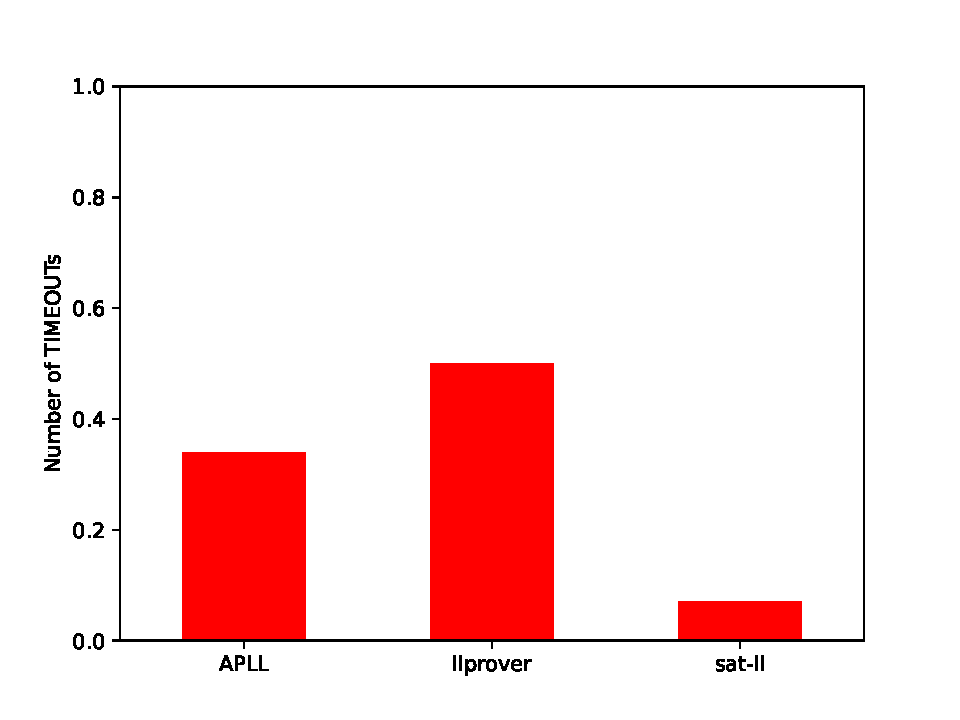
\includegraphics[scale=0.5]{./images/mll.pdf}
		\caption{Multiplicative case}
		\label{fig:mll-bars}
	\end{subfigure}
	\begin{subfigure}{0.49\textwidth}
		\centering
		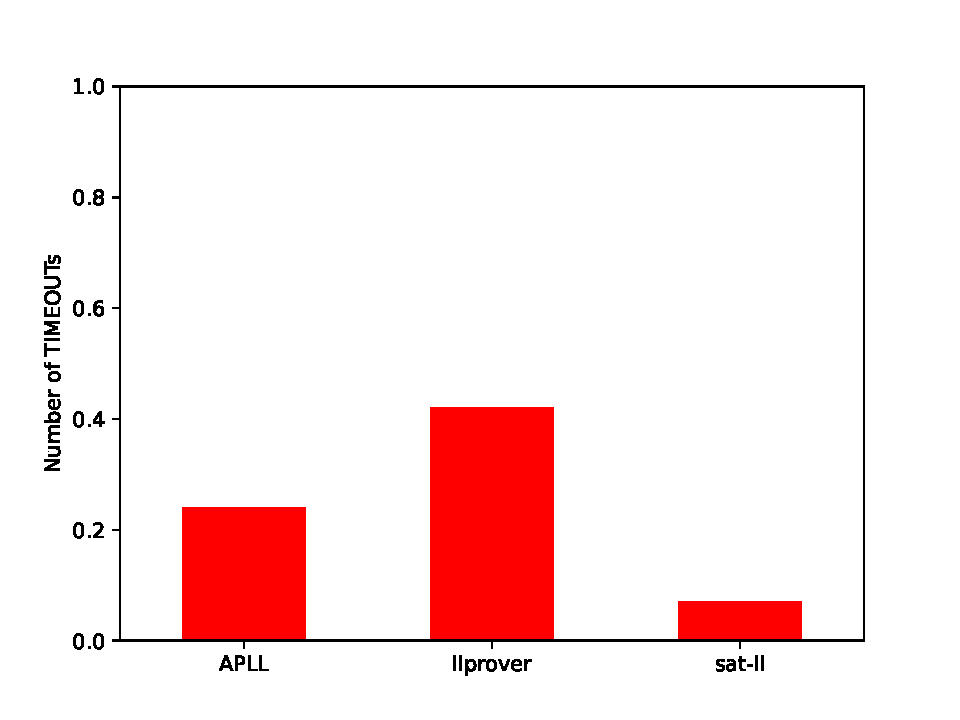
\includegraphics[scale=0.5]{./images/mall.pdf}
		\caption{Multiplicative and additive case}
		\label{fig:mall-bars}
	\end{subfigure}
	\caption{Percentage of number of timeouts out of a hundred formulae}
\end{figure}
We can see that in the multiplicative and additive case the difference begin to level.
The additive case is not that significant as the formulae remain manageable and no major differences can be seen.

As soon as exponentials come into play the differences level out.
\begin{figure}[h!]
	\centering
	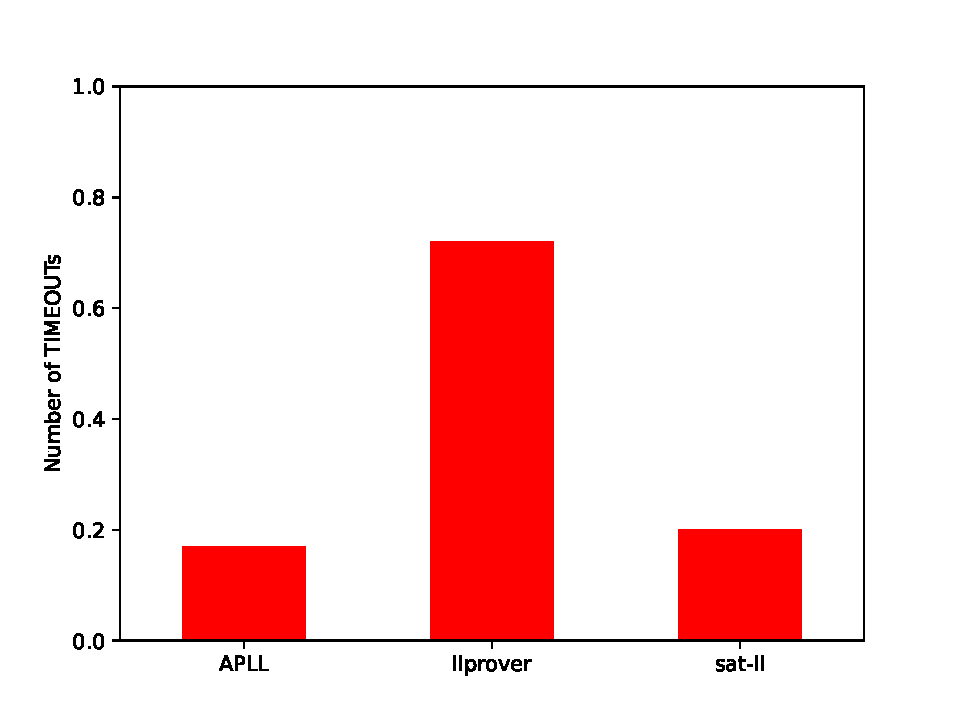
\includegraphics[scale=0.5]{./images/cll-500-250.pdf}
	\caption{Full linear logic}
	\label{fig:cll-bars}
\end{figure}
It can be seen in \ref{fig:cll-bars} that in full linear logic our prover performs slightly worse than APLL.

All these test were done generating suits of 100 tests.
Figure \ref{fig:mll-bars}'s tests were composed of normalized formulae of \texttt{size} 100, and \texttt{atoms} 50, with just the connectives $\llten$ and $\llpar$.
Figure \ref{fig:mall-bars}'s tests were composed of normalized formulae formulae of \texttt{size} 500, and \texttt{atoms} 250, with the connectives $\llten, \llpar, \llwith$ and $\llplus$.
Finally \ref{fig:cll-bars}'s tests were composed of normalized formulae of \texttt{size} 500, and \texttt{atoms} 250, with all the connectives.

When looking at the results of full linear logic, it is important to note that unlike the tests with multiplicatives and additives, some of the results may be early failures because of the bound.
Since llprover uses incremental search, its times are often the slowest.
Similarly our prover is consistently slightly slower that APLL, this difference is negligible and due to the fact that APLL is compiled, whereas our prover is interpreted.

\begin{table}[H]
	\centering
	\begin{tblr}{ 
		colspec = { l c c c c },
		vlines = {1,3,4,5,7,8,9,11,12,13}{solid},
		% cells = { preto = {\footnotesize} },
		% cells{2,7} = { preto = {\small}, cmd = {\textbf} }
		}
		\hline
		prover & timeouts & successes & success rate & avg. time (succ.) \\
		\hline
		\SetCell[c=5]{c} mll-100-50 \\
		\hline
		APLL & 34 & 66 & $0.66$ & \qty{1.441}{\second}  \\
		\hline
		llprover & 50 & 50 & $0.50$ & \qty{3.006}{\second}  \\
		\hline
		sat-ll & 7 & 93 & $0.93$ & \qty{1.874}{\second} \\
		\hline
		\SetCell[c=5]{c} mall-500-250 \\
		\hline
		APLL & 24 & 76 & $0.76 $ & \qty{1.213}{\second}  \\
		\hline
		llprover & 42 & 58 & $0.58$ & \qty{0.807}{\second}  \\
		\hline
		sat-ll & 7 & 93 & $0.93$ & \qty{1.289}{\second} \\
		\hline
		\SetCell[c=5]{c} cll-500-250 \\
		\hline
		APLL & 17 & 83 & $0.83 $ & \qty{0.967}{\second}  \\
		\hline
		llprover & 72 & 28 & $0.28 $ & \qty{0.409}{\second}  \\
		\hline
		sat-ll & 20 & 80 & $0.80 $ & \qty{1.940}{\second} \\
		\hline
	\end{tblr}
\end{table}

\bibliographystyle{plain}
\bibliography{refs}

\end{document}
